% Chapter 5. Every number here comes from a result file in the repository; the source is
% given in a comment above each table. Replace \pending items as results arrive.
\chapter{Results}
\label{ch:results}

The results follow the order of the stages. \Cref{sec:res-hex,sec:res-predictor} report on the
tools that the experiments depend on, and the remaining sections report experiments E1 to E5
(\cref{tab:experiments}) and the features of the best GQDs.

% ==========================================================================================
\section{Hexagon conversion}
\label{sec:res-hex}
% Source: Stage1/README.md (run of 2026-11-10)

All 91{,}174 dataset structures converted to hexagon lists, and converting each list back gave the
original canonical SMILES in every case. The structures have 20 to 40 hexagons. Of these,
14{,}674 have xTB values, with gaps from 0.00 to 2.03~eV; another 1{,}326 xTB results could not be
used because their structures were missing from the SMILES table. In a separate test, 3{,}000
random hexagon clusters with 1 to 45 rings and 3{,}000 dataset structures were converted in both
directions. There were no mismatches, and the result did not depend on the order in which the
hexagons were listed.

One limitation of RDKit appeared in these tests. For about 10 to 14\% of closed-shell random shapes
with 20 to 40 rings, our code finds a valid Kekul\'e structure, but RDKit cannot read back the
SMILES it writes for the molecule (its kekulisation search gives up). Such shapes are rejected
because every later step depends on RDKit. None of the 91{,}174 dataset structures is affected,
and about 3\% of LLM designs were.

% ==========================================================================================
\section{Gap predictor}
\label{sec:res-predictor}
% Source: Stage2/README.md, Stage2/results/metrics.json

\Cref{tab:predictor} shows the errors on the 1{,}468 held-out test GQDs. The H\"uckel baseline
alone reaches a mean absolute error (MAE) of 0.042~eV. The boosted trees reduce this to 0.031~eV,
and the graph network to 0.022~eV. The ensemble used in the workflow has an MAE of 0.023~eV and
\(R^2 = 0.981\). For comparison, the earlier model of the parent project had an MAE of 0.386~eV on
the same structures.

\begin{table}[ht]
  \centering
  \caption{Gap predictor on the held-out test set (1{,}468 GQDs never used in training or
           tuning).}
  \label{tab:predictor}
  \small
  \begin{tabular}{@{}lrrr@{}}
    \toprule
    Model & MAE (eV) & RMSE (eV) & \(R^2\) \\
    \midrule
    H\"uckel gap, linear fit only & 0.0421 & 0.0721 & 0.966 \\
    LightGBM (5 folds) & 0.0308 & 0.0638 & 0.974 \\
    XGBoost (5 folds) & 0.0307 & 0.0635 & 0.974 \\
    GNN (5 folds) & 0.0216 & 0.0542 & 0.981 \\
    Ensemble, 0.85 GNN + 0.15 XGBoost (used) & 0.0226 & 0.0549 & 0.981 \\
    \quad GQDs without holes (\(n = 1{,}344\)) & 0.0181 & 0.0441 & 0.988 \\
    \quad GQDs with holes (\(n = 124\)) & 0.0712 & 0.1208 & 0.863 \\
    \bottomrule
  \end{tabular}
\end{table}

The uncertainty is well calibrated: 96.7\% of test GQDs fall within \(\pm1.96\sigma\), against a
target of 95\%. The mean \(\sigma\) is 0.029~eV for GQDs without holes and 0.114~eV for GQDs with
holes, so the model reports larger uncertainty where its errors are larger. The rank correlation
between \(\sigma\) and the actual absolute error is 0.33. Errors grow modestly outside the training
distribution. For test gaps outside the central 90\% of the training gaps, the LightGBM MAE is
0.049~eV (H\"uckel baseline 0.064~eV), and a LightGBM model trained on GQDs with at most 34 hexagons
has an MAE of 0.033~eV on GQDs with 35 or more. Prediction takes about 4.5~s for 200 GQDs, most of
it spent starting the GNN process, and the full training took 78 minutes on the laptop CPU.

Structures with holes are four times harder to predict, and they make up 8.5\% of the data. This
was one of the reasons the evolutionary loop rejects holes (\cref{sec:loop}).

% ==========================================================================================
\section{E1: the LLM designs GQDs as hexagon lists}
\label{sec:res-e1}
% Source: Stage2d/README.md, Stage2d/results/ablation.md

In the first run (50 requests, basic prompt, plain feedback), 46\% of requests gave a valid GQD at
the first attempt and 64\% after up to two retries. Of the 67 failed attempts, 66 were open-shell
designs. The LLM wrote connected, duplicate-free lists of the right size, but it could not tell
which shapes have unequal sublattices, and the message ``no Kekul\'e form'' did not tell it what to
change.

\Cref{tab:e1} shows the ablation. Each aid helps in a different way. The closed-shell rule in the
prompt raises the first-attempt pass rate from 34\% to 56\% (plain feedback) and 57\% (fix edits), because fewer designs are
open-shell to begin with. The fix edits make retries work: with the basic prompt they raise the
final pass rate from 52\% to 90\%. With both aids, 79 of 80 requests (99\%) ended in a valid GQD,
the mean number of attempts fell from 2.21 to 1.53, and open-shell attempts fell from 131 to 39.
Shapes that had almost always failed now succeeded: with both aids, L-shaped, triangular and
irregular requests went from 1, 3 and 0 valid designs out of 10 to 10 out of 10 each. Almost all
valid designs were new compared with the dataset, and none had holes.

\begin{table}[ht]
  \centering
  \caption{E1 ablation: 80 identical requests per condition, up to two retries. Prompt: basic or
           with the closed-shell rule. Feedback: plain or with fix edits.}
  \label{tab:e1}
  \small
  \begin{tabular}{@{}lrrrr@{}}
    \toprule
    & basic, plain & basic, fixes & rule, plain & rule, fixes \\
    \midrule
    Valid at first attempt & 34\% & 36\% & 56\% & 57\% \\
    Valid after \(\leq 2\) retries & 52\% & 90\% & 82\% & \textbf{99\%} \\
    Mean attempts per request & 2.21 & 1.83 & 1.66 & 1.53 \\
    Failed attempts: open-shell & 131 & 67 & 63 & 39 \\
    Failed attempts: other reasons & 4 & 7 & 4 & 4 \\
    Valid designs & 42 & 72 & 66 & 79 \\
    Distinct valid designs & 33 & 67 & 45 & 55 \\
    Most repeated design & \(\times 4\) & \(\times 2\) & \(\times 11\) & \(\times 9\) \\
    New compared with the dataset & 42/42 & 70/72 & 66/66 & 79/79 \\
    Point-symmetric & 45\% & 24\% & 58\% & 48\% \\
    Mean size error (hexagons) & 0.4 & 0.9 & 1.7 & 1.9 \\
    Predicted gap range (eV) & 0.05--1.42 & 0.02--1.27 & 0.07--1.40 & 0.01--1.51 \\
    \bottomrule
  \end{tabular}
\end{table}

The rule prompt has a cost. With it, the LLM often fell back on a standard symmetric shape: one
design appeared 11 times in 80 requests with plain feedback and 9 times with fix edits. The fix
edits alone kept the most variety (67 distinct designs out of 72 valid ones). Designs also drifted
from the requested size by about two hexagons when fixes or symmetry were applied, though they
always stayed within 20 to 40. In the agent, repeats are caught by the uniqueness check, and in
the evolutionary loop variety comes from editing different parents.

LLM results vary between runs. The basic-prompt, plain-feedback condition gave 46\% and 64\% in
the first run and 34\% and 52\% when repeated in the ablation. Conditions should therefore be
compared within the same run, as in \cref{tab:e1}.

% ==========================================================================================
\section{E2: the sensing score on 50 dataset GQDs}
\label{sec:res-e2}
% Source: Stage3a/README.md, Stage3a/results/summary.md, Stage3a/data/calibration.csv

\subsection{A geometry problem found and fixed}
\label{sec:res-flat}

The first calibration run started every GQD perfectly flat. Nearly all dataset GQDs have crowded
edges, coves or fjords, in 48 of the 50 sampled here, and their relaxed shape is twisted. A flat
start has no force out of the plane, so the optimiser kept these GQDs flat and strained. When a gas
was added, it broke the symmetry, the GQD twisted and released its strain, and the released energy
was counted as adsorption energy. In the worst case water appeared to bind by \(-6.3\)~eV. With
the small random out-of-plane displacement (\cref{sec:score}), 48 of the 50 GQDs relaxed to
structures more than 0.5~\AA{} out of plane, and the xTB gaps of our optimised GQDs agreed with the
dataset gaps with a mean absolute difference of 0.036~eV (\(r = 0.984\)). The flawed run is kept
in the repository for reference, and all results below come from the corrected run.

\subsection{Descriptors}

All 50 evaluations finished and every optimisation converged. \Cref{tab:calibration} groups the
results by gap, and \cref{fig:sensing-vs-gap} shows them for every GQD.

\begin{table}[ht]
  \centering
  \caption{E2: \ce{NO2} sensing descriptors of 50 dataset GQDs (10 per gap range; medians unless
           stated). Adsorption energies in eV, charge in \(e\).}
  \label{tab:calibration}
  \small
  \begin{tabular}{@{}lccccc@{}}
    \toprule
    Gap (eV) & \(E_{\ce{NO2}}\) & Chemisorbed & \(q_{\ce{NO2}}\) & \ce{H2O} / \ce{NH3} / CO & Score, median (max) \\
    \midrule
    0.0--0.4 & \(-1.15\) & 9/10 & 0.21 & \(-0.13\) / \(-0.14\) / \(-0.23\) & 0.00 (0.28) \\
    0.4--0.8 & \(-0.66\) & 7/10 & 0.21 & \(-0.14\) / \(-0.14\) / \(-0.24\) & 0.18 (0.32) \\
    0.8--1.2 & \(-0.38\) & 3/10 & 0.22 & \(-0.15\) / \(-0.16\) / \(-0.25\) & 0.22 (0.26) \\
    1.2--1.6 & \(-0.62\) & 6/10 & 0.22 & \(-0.15\) / \(-0.15\) / \(-0.25\) & 0.12 (0.25) \\
    1.6--2.1 & \(-0.34\) & 4/10 & 0.19 & \(-0.15\) / \(-0.16\) / \(-0.23\) & 0.15 (0.20) \\
    \bottomrule
  \end{tabular}
\end{table}

\begin{figure}[ht]
  \centering
  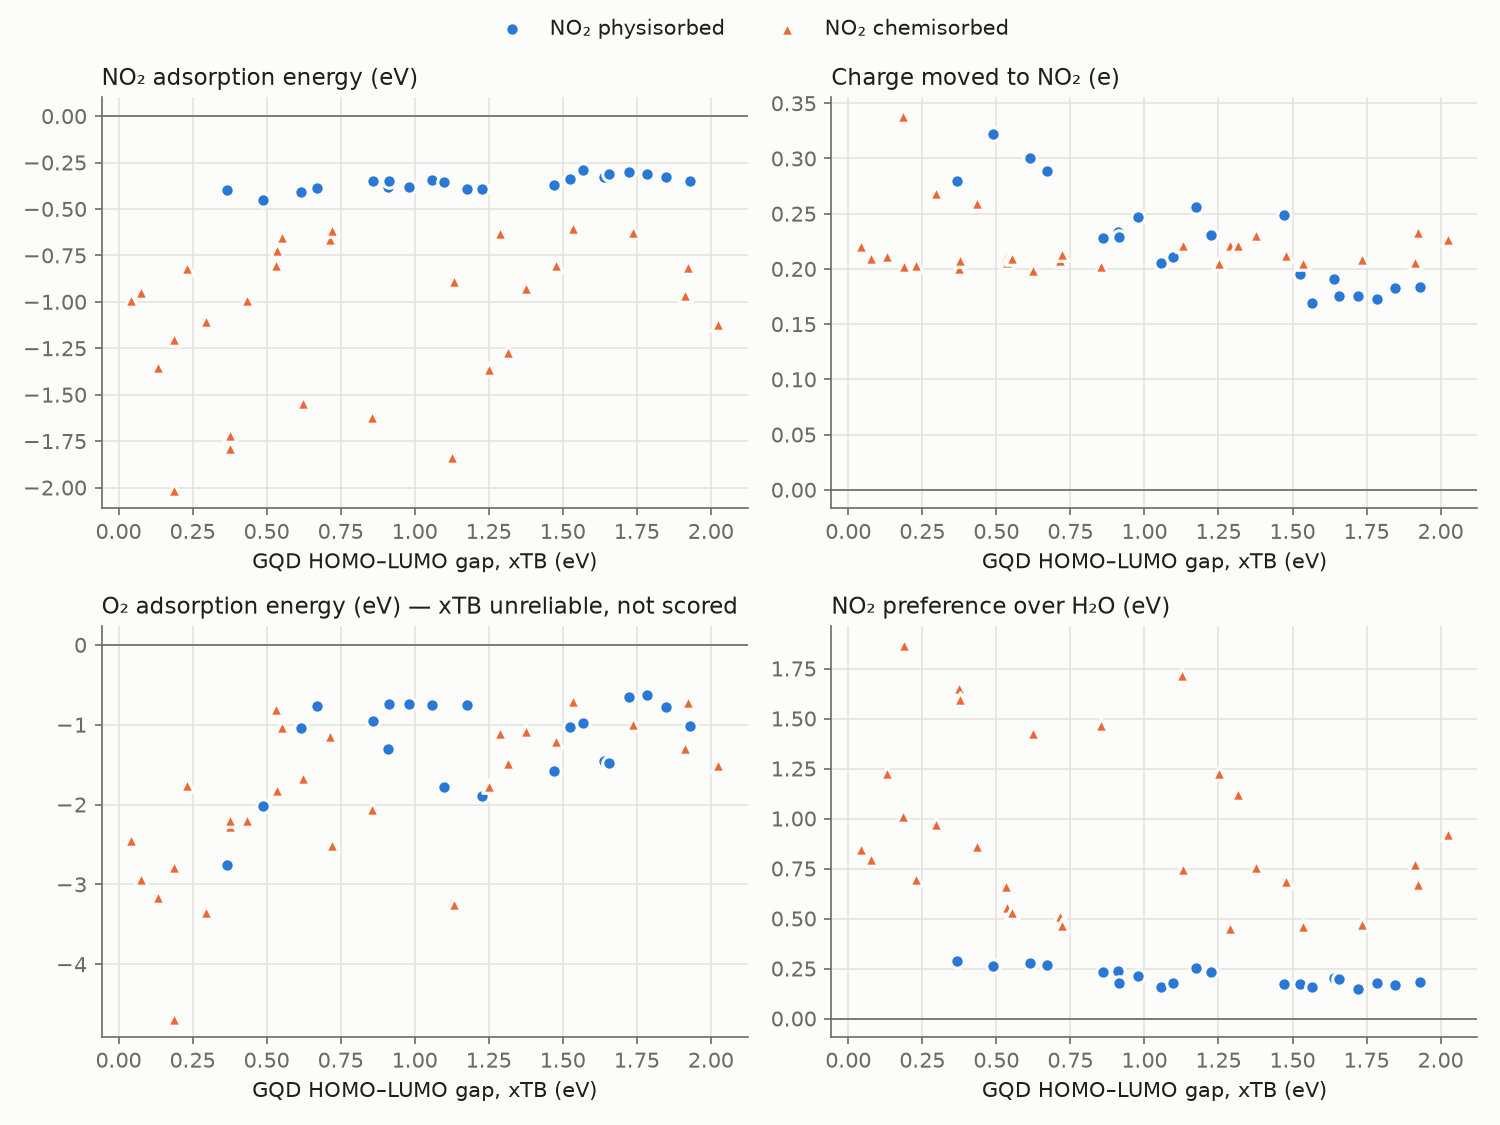
\includegraphics[width=\textwidth]{stage3a_sensing_vs_gap.png}
  \caption{E2: descriptors of the 50 calibration GQDs against their xTB gap. Circles: \ce{NO2}
           physisorbed; triangles: \ce{NO2} chemisorbed (contact shorter than 1.9~\AA). Top left:
           \ce{NO2} adsorption energy. Top right: charge moved to \ce{NO2}. Bottom left: \ce{O2}
           adsorption energy, which xTB describes wrongly and which is not scored. Bottom right:
           how much more strongly \ce{NO2} binds than \ce{H2O}.}
  \label{fig:sensing-vs-gap}
\end{figure}

\ce{NO2} binds in two distinct ways. In 21 of the 50 GQDs it physisorbs, at \(-0.29\) to
\(-0.45\)~eV, which corresponds to a recovery time well below one second. In the other 29 a
carbon-nitrogen bond forms, and xTB gives \(-0.6\) to \(-2.0\)~eV. Chemisorption is much more
common at small gaps (9 of 10 GQDs below 0.4~eV) but occurs at every gap, because it depends on the
local site rather than on the GQD as a whole. Simple structural features predicted it only weakly;
the best single predictors (many isolated edge \ce{C-H} groups, fewer Kekul\'e structures and a smaller
gap) reached an area under the ROC curve of at most 0.73.

For physisorbed \ce{NO2}, the charge moved to \ce{NO2} grows as the gap shrinks, from about
0.17~\(e\) at a gap of 1.9~eV to about 0.32~\(e\) at 0.5~eV. A smaller gap goes with a higher HOMO,
so the GQD gives up electrons more easily. Selectivity among the interfering gases was never the
limiting factor. CO was the strongest competitor in all 50 GQDs, but \ce{NO2} always bound more
strongly, by 0.1 to 0.2~eV in the physisorbed GQDs.

\subsection{Score}

Thirty-eight of the 50 GQDs scored above zero (\cref{fig:score-vs-gap}). The best scores, 0.28 to
0.32, all came from GQDs that physisorb \ce{NO2} and have a gap of about 0.35 to 0.7~eV. The three
best were \code{gqd\_18941} (score 0.32, gap 0.49~eV), \code{gqd\_23821} (0.30, 0.61~eV) and
\code{gqd\_90531} (0.29, 0.67~eV). This range is also where the trade-off is sharpest: 7 of the 10
dataset GQDs with gaps between 0.4 and 0.8~eV chemisorb \ce{NO2} and score low. Finding a GQD with a
small gap that still physisorbs \ce{NO2} is therefore the actual design problem, and it became the
goal of the evolutionary loop.

\begin{figure}[ht]
  \centering
  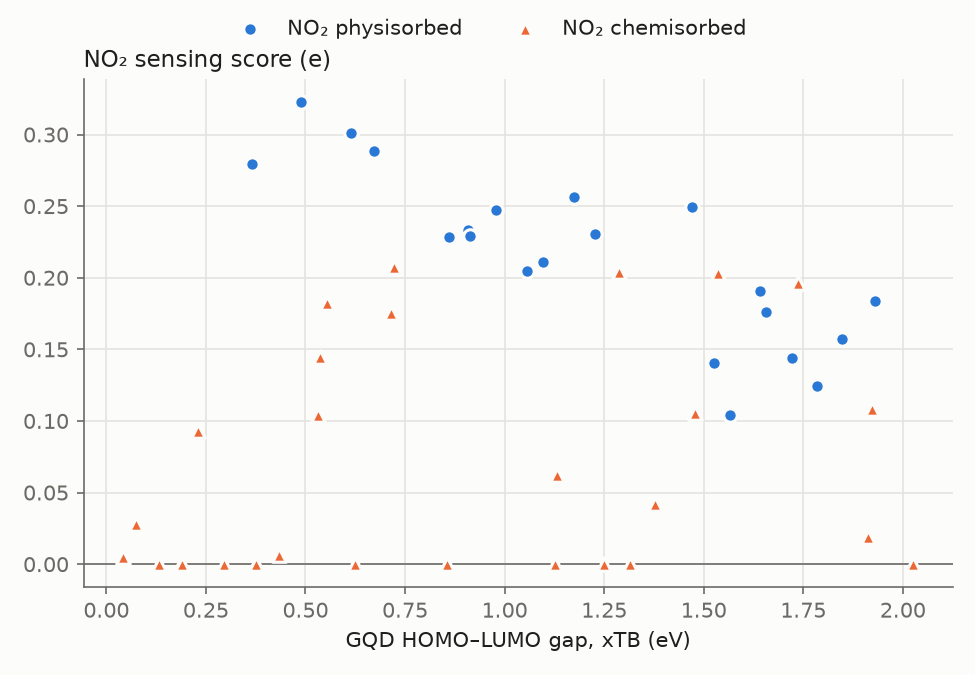
\includegraphics[width=0.8\textwidth]{stage3a_score_vs_gap.png}
  \caption{E2: \ce{NO2} sensing score of the 50 calibration GQDs against their xTB gap. The best
           scores come from physisorbing GQDs with gaps of about 0.35 to 0.7~eV. Chemisorbing GQDs
           (triangles) are penalised by the reversibility factor.}
  \label{fig:score-vs-gap}
\end{figure}

% ==========================================================================================
\section{E3: xTB against DFT on small models}
\label{sec:res-dft-small}
% Source: Stage3a/README.md, Stage3a/data/dft_check/

\Cref{tab:dft-tetracene,tab:dft-coronene} compare xTB and DFT at the same geometries.

\begin{table}[ht]
  \centering
  \caption{E3: tetracene, on which xTB chemisorbs \ce{NO2}. Energies in eV, charges on the gas in
           \(e\) (xTB charges; meta-L\"owdin for DFT).}
  \label{tab:dft-tetracene}
  \small
  \begin{tabular}{@{}lrrrrr@{}}
    \toprule
    Complex & Distance (\AA) & \(\Eads\) xTB & \(\Eads\) DFT & \(q\) xTB & \(q\) DFT \\
    \midrule
    \ce{NO2}, centre (chemisorbed) & 1.52 & \(-1.20\) & \(-0.76\) & 0.20 & 0.19 \\
    \ce{NO2}, edge (chemisorbed) & 1.53 & \(-0.74\) & \(-0.19\) & 0.19 & 0.19 \\
    \ce{NO2}, O down (chemisorbed) & 1.47 & \(-0.68\) & \(-0.59\) & 0.26 & 0.27 \\
    \ce{O2}, centre & 1.45 & \(-1.52\) & \(+0.53\) & 0.34 & 0.28 \\
    \ce{O2}, edge & 1.46 & \(-1.07\) & \(+1.10\) & 0.36 & 0.28 \\
    \ce{H2O} & 2.69 & \(-0.12\) & \(-0.24\) & 0.01 & 0.01 \\
    \bottomrule
  \end{tabular}
\end{table}

\begin{table}[ht]
  \centering
  \caption{E3: coronene, on which xTB physisorbs \ce{NO2}. Units as in \cref{tab:dft-tetracene}.}
  \label{tab:dft-coronene}
  \small
  \begin{tabular}{@{}lrrrrr@{}}
    \toprule
    Complex & Distance (\AA) & \(\Eads\) xTB & \(\Eads\) DFT & \(q\) xTB & \(q\) DFT \\
    \midrule
    \ce{NO2}, centre & 3.06 & \(-0.19\) & \(-0.20\) & 0.04 & 0.00 \\
    \ce{NO2}, edge & 2.55 & \(-0.24\) & \(-0.06\) & 0.13 & 0.04 \\
    \ce{NO2}, O down, centre & 2.87 & \(-0.18\) & \(-0.20\) & 0.09 & 0.00 \\
    \ce{NO2}, O down, edge & 2.75 & \(-0.18\) & \(-0.20\) & 0.09 & 0.00 \\
    \ce{O2}, edge & 2.62 & \(-0.51\) & \(+0.23\) & 0.30 & 0.03 \\
    \ce{O2}, centre & 2.59 & \(-0.47\) & \(+3.74\)\(^{a}\) & 0.30 & 0.36\(^{a}\) \\
    CO, centre / edge & 3.2 & \(-0.09\) / \(-0.07\) & \(-0.08\) / \(-0.06\) & 0.01 & 0.01 \\
    \ce{NH3}, centre / edge & 2.9 & \(-0.14\) / \(-0.13\) & \(-0.22\) / \(-0.19\) & 0.00 & 0.00 \\
    \ce{H2O}, centre / edge & 2.7 & \(-0.13\) / \(-0.12\) & \(-0.26\) / \(-0.24\) & 0.01 & 0.01 \\
    \bottomrule
    \multicolumn{6}{@{}l}{\footnotesize \(^{a}\) Probably converged to a wrong, charge-separated
      electronic state. \ce{O2} is unbound in DFT either way.}
  \end{tabular}
\end{table}

Four findings follow. First, for the closed-shell gases and for physisorbed \ce{NO2}, xTB
adsorption energies are close to DFT, mostly within 0.1~eV. The larger DFT binding of \ce{H2O}
(\(-0.24\) to \(-0.26\)~eV) is consistent with the overbinding expected from the small basis set
without counterpoise correction. Second, the \ce{NO2} chemisorption seen in xTB is real, since DFT
also binds the bonded complexes, but xTB overbinds them by 0.1 to 0.55~eV. Third, the charge moved
to \ce{NO2} agrees within about 0.01~\(e\) for chemisorbed \ce{NO2}, but for physisorbed \ce{NO2}
xTB overestimates it (0.04 to 0.13~\(e\) against 0.00 to 0.04~\(e\) on coronene). This is the
over-delocalisation expected from a DFT-like method \cite{cohen2008insights}. Across the 21
physisorbing calibration GQDs, the xTB charge still follows the GQD's HOMO energy closely
(\(r = 0.88\)), and a higher HOMO means a better electron donor, which is the physically expected
direction. The response term therefore ranks GQDs sensibly, but its absolute values for
physisorption are too large. Fourth, xTB binds \ce{O2} (\(-0.5\) to \(-1.5\)~eV), while DFT finds
it unbound in every case. \ce{O2} was therefore left out of the score, and the air stability of
the final candidates has to be checked with DFT.

% ==========================================================================================
\section{E5a: pilot comparison of LLM and random mutation}
\label{sec:res-pilot}
% Source: Stage3/README.md, Stage3/results/compare.md, Stage3/results/{llm_s0,random_s0}/

Both pilot runs started from the same population (best score 0.322) and took about 55 minutes
each on the laptop. \Cref{tab:pilot} summarises them and \cref{fig:pilot} shows their progress.

\begin{table}[ht]
  \centering
  \caption{E5a: pilot runs, 10 generations, one run per mutator (seed 0, loop version 1).}
  \label{tab:pilot}
  \small
  \begin{tabular}{@{}lrr@{}}
    \toprule
    & LLM & random \\
    \midrule
    Children proposed & 300 & 300 \\
    Valid (passed all checks) & 31\% & 54\% \\
    Scored by xTB & 80 & 100 \\
    Scored children that beat their parent & 11\% & 11\% \\
    Scored children with chemisorbed \ce{NO2} & 35\% & 47\% \\
    Mean score of scored children & 0.211 & 0.190 \\
    Best score & \textbf{0.340} & 0.331 \\
    Children above the best starting score (0.322) & 10 & 9 \\
    \bottomrule
  \end{tabular}
\end{table}

\begin{figure}[ht]
  \centering
  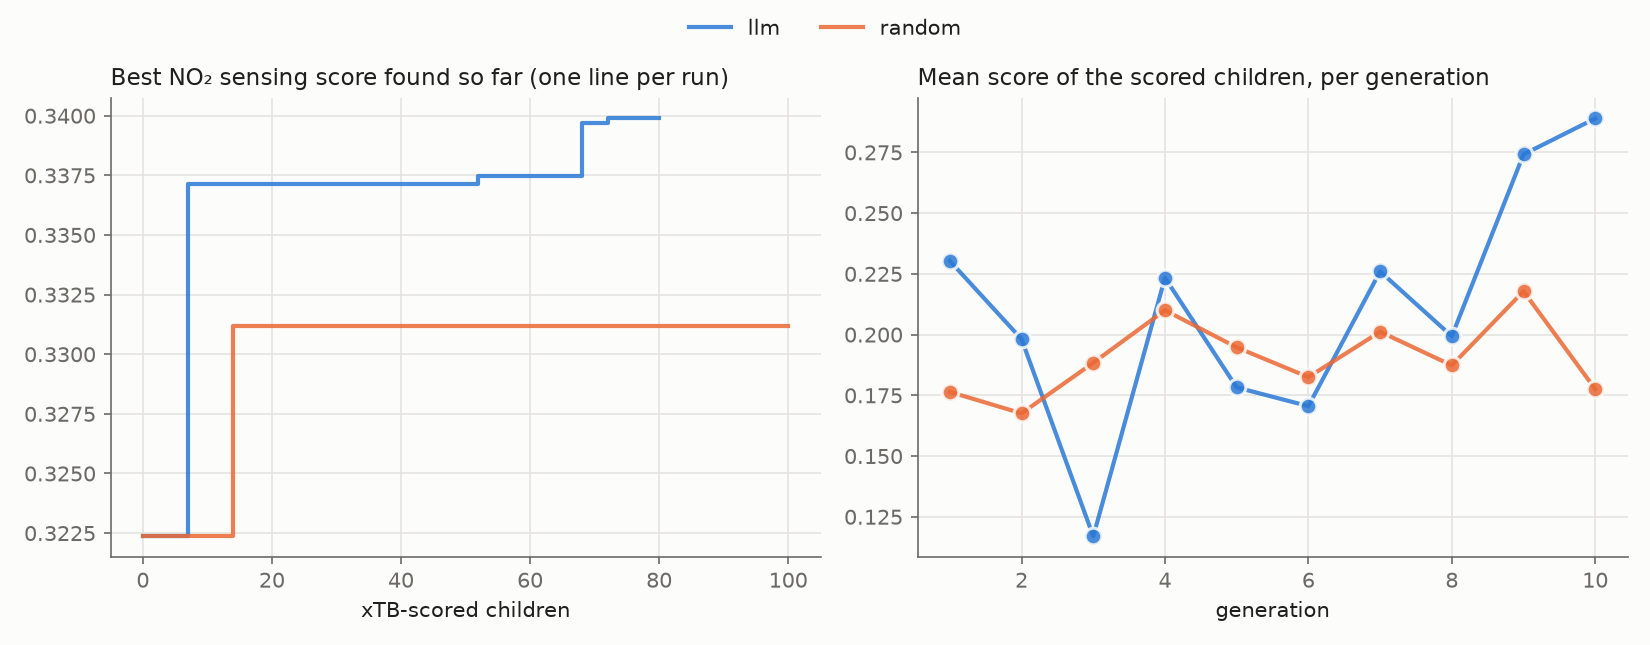
\includegraphics[width=\textwidth]{stage3_pilot_compare.png}
  \caption{E5a: pilot runs. Left: best score found so far against the number of xTB-scored
           children (the vertical axis is zoomed in). Right: mean score of the scored children in
           each generation.}
  \label{fig:pilot}
\end{figure}

The LLM run found the best GQD (0.340 against 0.331) with fewer xTB evaluations. It passed the best
starting score after 7 scored children, against 14 for the random run, and its children
chemisorbed \ce{NO2} less often. Its mean score per generation rose in the last two generations
(0.27 to 0.29, against 0.18 to 0.22 for random). With one run per mutator, however, the difference
in scores is not significant (one-sided Mann-Whitney \(p = 0.20\) on the scores of all scored
children), and the gain over the start, 0.018, is about the size of the noise from xTB and from
probing only two sites.

The ten best new GQDs (five per run) were scored again with all five gases. The loop score
matched the full score within 0.002 in every case, CO was always the strongest competing gas, and
\ce{NO2} bound more strongly than \ce{H2O} by at least 0.27~eV. \Cref{tab:pilot-best} lists the
best of them. All physisorb \ce{NO2}. The LLM's best GQDs have gaps of 0.29 to 0.33~eV, smaller
than any of the best calibration GQDs, while still physisorbing \ce{NO2}.

\begin{table}[ht]
  \centering
  \caption{E5a: best GQDs of the pilot runs after the full check with all gases. Margins are
           \(E_g - E_{\ce{NO2}}\) for CO and \ce{H2O}; positive means \ce{NO2} binds more strongly.}
  \label{tab:pilot-best}
  \small
  \begin{tabular}{@{}llrrrrrrr@{}}
    \toprule
    GQD & Run & Hexagons & Gap & \(E_{\ce{NO2}}\) & \(q_{\ce{NO2}}\) & CO margin & \ce{H2O} margin & Score \\
        &     &          & (eV) & (eV) & (\(e\)) & (eV) & (eV) & (\(e\)) \\
    \midrule
    g10c004 & LLM & 38 & 0.29 & \(-0.50\) & 0.34 & \(+0.25\) & \(+0.31\) & 0.341 \\
    g10c007 & LLM & 37 & 0.30 & \(-0.50\) & 0.34 & \(+0.25\) & \(+0.31\) & 0.340 \\
    g09c019 & LLM & 38 & 0.33 & \(-0.49\) & 0.34 & \(+0.25\) & \(+0.33\) & 0.340 \\
    g07c026 & LLM & 36 & 0.30 & \(-0.49\) & 0.34 & \(+0.24\) & \(+0.31\) & 0.338 \\
    g01c022 & LLM & 35 & 0.31 & \(-0.49\) & 0.34 & \(+0.25\) & \(+0.30\) & 0.337 \\
    g02c004 & random & 35 & 0.36 & \(-0.49\) & 0.33 & \(+0.24\) & \(+0.30\) & 0.331 \\
    g07c013 & random & 33 & 0.45 & \(-0.47\) & 0.33 & \(+0.22\) & \(+0.28\) & 0.331 \\
    \bottomrule
  \end{tabular}
\end{table}

The pilot also exposed three problems with the loop.
\begin{enumerate}
  \item \emph{Low validity of LLM children (31\%).} Of the 300 LLM proposals, 100 were
        open-shell, partly because the LLM often used two or three edits per child, while the
        random mutator mostly used one. Another 43 were duplicates, about 30 contained bookkeeping
        errors (adding a hexagon that was already there or removing one that was not), and 10 used
        four edits. As a result, 6 of the 10 LLM generations scored fewer than 10 children.
  \item \emph{Loss of diversity.} By generation 10, all eight LLM parents descended from one
        starting GQD (\code{gqd\_14650}). The random run kept two families.
  \item \emph{Gap floor.} The LLM's best GQDs sat at the lower edge of the 0.30~eV pre-filter, and
        about 10 LLM children were skipped for a predicted gap below 0.30~eV.
\end{enumerate}
These problems led to version 2 of the loop (\cref{tab:loop-versions}). Applied to the pilot's
proposals, the open-shell repair alone would have raised validity from 31\% to 50\% for the LLM
and from 54\% to 81\% for random mutation. In addition, xTB gave \ce{O2} adsorption energies of
\(-2.7\) to \(-3.4\)~eV for the best GQDs, which is consistent with the known \ce{O2} error of xTB
(\cref{sec:res-dft-small}) but means that air stability must be checked with DFT.

% ==========================================================================================
\section{E5b: main comparison of LLM and random mutation}
\label{sec:res-main}
% Source: Stage3/results/compare_v2.md and compare_v2.png, made by
%   Stage3/compare.py llm_v2_s1 llm_v2_s2 llm_v2_s3 random_v2_s1 random_v2_s2 random_v2_s3 --name v2
% from Stage3/results/{llm,random}_v2_s{1,2,3}/children.jsonl; LLM calls from llm_log.jsonl;
% full checks from final_check.csv. random_v2_s3 was interrupted after generation 5 and resumed
% with the same seed.

All six runs of loop version 2 finished. \Cref{tab:main} gives the result of each run,
\cref{tab:main-mutator} the mean and standard deviation over the three runs of each mutator, and
\cref{fig:main} the progress of each run.

\begin{table}[ht]
  \centering
  \caption{E5b: the six runs of loop version 2 (10 generations each, seeds 1 to 3). ``Repaired'' is
           the share of all proposals that became valid only after repair by code.}
  \label{tab:main}
  \small
  \begin{tabular}{@{}lrrrrrr@{}}
    \toprule
    & \multicolumn{3}{c}{LLM} & \multicolumn{3}{c}{random} \\
    \cmidrule(lr){2-4}\cmidrule(l){5-7}
    & s1 & s2 & s3 & s1 & s2 & s3 \\
    \midrule
    Children proposed & 207 & 255 & 191 & 300 & 300 & 300 \\
    Valid & 59\% & 45\% & 60\% & 84\% & 84\% & 79\% \\
    Repaired by code & 39\% & 28\% & 41\% & 33\% & 33\% & 32\% \\
    Scored by xTB & 99 & 100 & 100 & 100 & 100 & 100 \\
    Beat their parent & 13\% & 12\% & 7\% & 13\% & 9\% & 5\% \\
    \ce{NO2} chemisorbed & 49\% & 54\% & 51\% & 52\% & 65\% & 60\% \\
    Mean score of scored children & 0.194 & 0.172 & 0.191 & 0.178 & 0.157 & 0.154 \\
    Best score & 0.342 & 0.343 & 0.348 & \textbf{0.356} & 0.354 & 0.341 \\
    Children above 0.322 & 6 & 2 & 5 & 4 & 2 & 4 \\
    LLM calls & 27 & 34 & 20 & n/a & n/a & n/a \\
    \bottomrule
  \end{tabular}
\end{table}

\begin{table}[ht]
  \centering
  \caption{E5b: mean \(\pm\) standard deviation over the three runs of each mutator.}
  \label{tab:main-mutator}
  \small
  \begin{tabular}{@{}lrrr@{}}
    \toprule
    Mutator & Best score & Mean score of scored children & Valid \\
    \midrule
    LLM & \(0.344 \pm 0.004\) & \(0.186 \pm 0.012\) & 55\% \\
    random & \(0.351 \pm 0.008\) & \(0.163 \pm 0.013\) & 82\% \\
    \bottomrule
  \end{tabular}
\end{table}

\begin{figure}[ht]
  \centering
  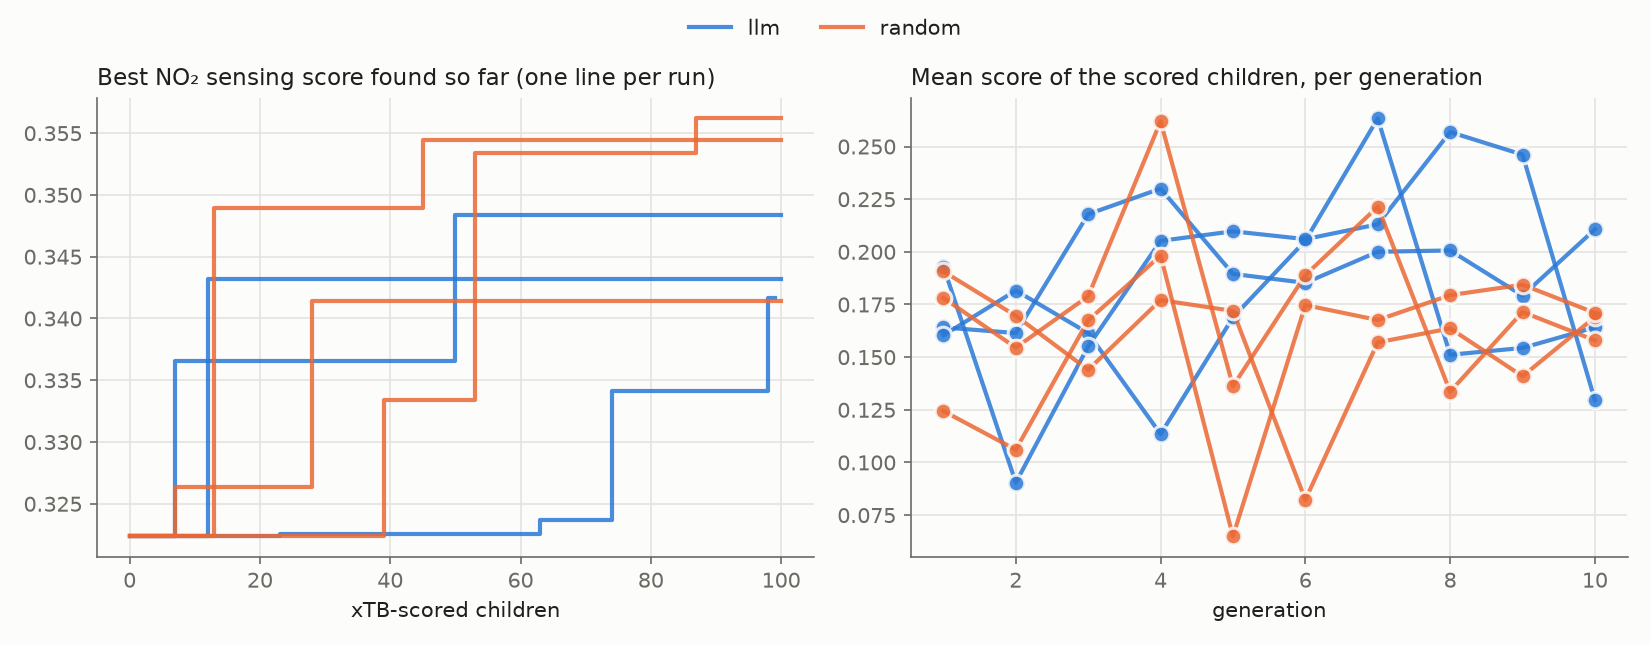
\includegraphics[width=\textwidth]{stage4_compare_v2.png}
  \caption{E5b: the six runs of loop version 2, one line per run. Left: best score found so far
           against the number of xTB-scored children (the vertical axis is zoomed in). Right: mean
           score of the scored children in each generation.}
  \label{fig:main}
\end{figure}

The changes of version 2 did what they were meant to do. Every run used the whole xTB budget (99
or 100 children, against 80 for the LLM in the pilot). Validity rose from 31\% to between 45\% and
60\% for the LLM and from 54\% to between 79\% and 84\% for random mutation, and in both cases a
large part of the valid children were open-shell proposals that the code repaired. Because more
proposals were valid, the LLM runs needed fewer of them (191 to 255, against 300 in the pilot) and
20 to 34 LLM calls per run. The full check with all gases confirmed the loop scores within 0.003
for all 30 GQDs checked. CO was the strongest competing gas for 27 of them; for the other three,
all from random runs, \ce{NH3} bound 0.001~eV more strongly than CO, which does not change their
scores.

The two mutators differ in a consistent way, but not in the way H3 predicted. Random mutation found
the best single GQD in two of the three seed pairs (0.356 and 0.354, against 0.342 and 0.343 for
the LLM), and the LLM did so in the third (0.348 against 0.341). The mean best score is 0.351 for
random mutation and 0.344 for the LLM, a difference of 0.007 that is smaller than the spread
between runs of the same mutator. On the best score, the LLM therefore shows no advantage. The mean
score of the scored children, however, was higher for the LLM in all three pairs (0.194, 0.172 and
0.191, against 0.178, 0.157 and 0.154), and its children chemisorbed \ce{NO2} less often in all
three (49 to 54\%, against 52 to 65\%). A one-sided Mann-Whitney test on the scores of all scored
children gives \(p = 0.004\) in favour of the LLM (299 against 300 children). As explained in
\cref{sec:e5}, children of one run are not independent, so this value overstates the evidence. The
number of xTB evaluations needed to pass the starting best was similar for the two mutators (23,
12 and 7 for the LLM; 39, 13 and 7 for random mutation).

In short, the LLM's proposals are better on average and avoid chemisorption somewhat more often,
while random mutation, with its larger variety of edits, found the two highest-scoring GQDs of the
study. H3 is supported for the mean score and not supported for the best score.

% ==========================================================================================
\section{E4: xTB against DFT on twelve GQDs}
\label{sec:res-e4}
% Source: Stage3a/results/dft_benchmark.md and dft_benchmark.csv (made by
% Stage3a/analyze_dft_benchmark.py from Stage3a/data/dft_benchmark/summary.csv and <gqd>/dft.csv)

All 162 single points finished and every SCF converged. \Cref{tab:e4-rho} compares the two methods
across the twelve GQDs, \cref{tab:e4-complex} compares the individual complexes, and
\cref{fig:e4-parity} shows the three quantities that make up the score.

\begin{table}[ht]
  \centering
  \caption{E4: xTB against DFT across the 12 benchmark GQDs. Each quantity is taken at the site
           and orientation where the method finds the strongest binding. The margin is the
           preference for \ce{NO2} over the strongest interfering gas.}
  \label{tab:e4-rho}
  \small
  \begin{tabular}{@{}lrrrr@{}}
    \toprule
    Quantity & Spearman \(\rho\) & Pearson \(r\) & MAE & Mean DFT \(-\) xTB \\
    \midrule
    \(E_{\ce{NO2}}\) (eV) & 0.74 & 0.87 & 0.223 & \(+0.035\) \\
    \(E_{\ce{H2O}}\) (eV) & 0.85 & 0.88 & 0.220 & \(-0.220\) \\
    \(E_{\ce{NH3}}\) (eV) & 0.95 & 0.94 & 0.144 & \(-0.144\) \\
    \(E_{\ce{CO}}\) (eV) & 0.10 & 0.12 & 0.330 & \(+0.330\) \\
    \(E_{\ce{O2}}\) (eV) & \(-0.44\) & \(-0.28\) & 1.840 & \(+1.840\) \\
    Selectivity margin (eV) & 0.86 & 0.90 & 0.269 & \(-0.167\) \\
    \(q_{\ce{NO2}}\) (\(e\)) & \(-0.11\) & \(-0.45\) & 0.185 & \(-0.185\) \\
    Sensing score (\(e\)) & \(-0.16\) & \(-0.15\) & 0.180 & \(-0.180\) \\
    \bottomrule
  \end{tabular}
\end{table}

\begin{table}[ht]
  \centering
  \caption{E4: individual complexes, grouped by the xTB geometry (bonded if the shortest contact is
           below 1.9~\AA) and by the DFT electronic state (charge-separated if more than 0.3~\(e\)
           sits on the gas). Means of adsorption energy (eV) and of the charge moved to the gas
           (\(e\)).}
  \label{tab:e4-complex}
  \small
  \begin{tabular}{@{}lllrrrrr@{}}
    \toprule
    Gas & Geometry & DFT state & \(n\) & \(\Eads\) xTB & \(\Eads\) DFT & Charge xTB & Charge DFT \\
    \midrule
    \ce{NO2} & physisorbed & neutral & 34 & \(-0.32\) & \(-0.26\) & 0.23 & 0.01 \\
    \ce{NO2} & physisorbed & charge-separated & 7 & \(-0.44\) & \(+0.52\) & 0.32 & 0.60 \\
    \ce{NO2} & bonded & neutral & 7 & \(-0.90\) & \(-0.73\) & 0.23 & 0.21 \\
    \ce{O2} & physisorbed & neutral & 12 & \(-0.69\) & \(+0.33\) & 0.39 & 0.05 \\
    \ce{O2} & bonded & both & 11 & \(-1.88\) & \(+0.88\) & 0.43 & 0.39 \\
    \ce{H2O} & physisorbed & neutral & 24 & \(-0.14\) & \(-0.32\) & 0.01 & 0.00 \\
    \ce{NH3} & physisorbed & neutral & 24 & \(-0.15\) & \(-0.26\) & 0.00 & \(-0.01\) \\
    CO & physisorbed & neutral & 24 & \(-0.21\) & \(+0.12\) & 0.07 & 0.05 \\
    \bottomrule
  \end{tabular}
\end{table}

\begin{figure}[ht]
  \centering
  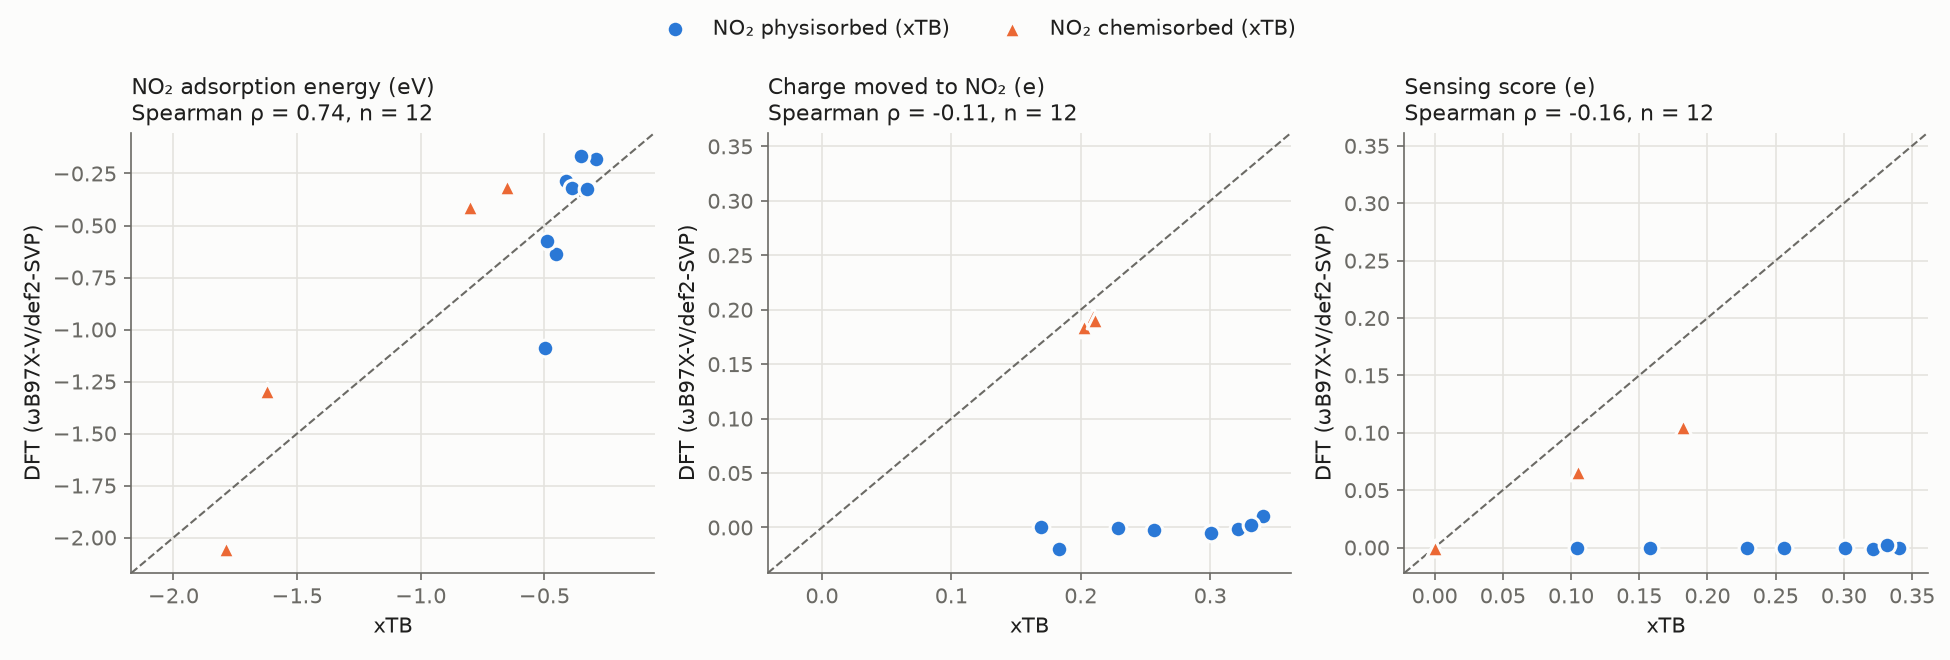
\includegraphics[width=\textwidth]{stage4_dft_vs_xtb.png}
  \caption{E4: xTB against DFT for the 12 benchmark GQDs. Left: \ce{NO2} adsorption energy.
           Middle: charge moved to \ce{NO2}. Right: sensing score. Circles: \ce{NO2} physisorbed in
           the xTB geometry; triangles: bonded. The dashed line is \(y = x\).}
  \label{fig:e4-parity}
\end{figure}

\paragraph{Binding energies are ranked well.} xTB and DFT order the GQDs in nearly the same way
for the binding of \ce{NO2} (\(\rho = 0.74\)), \ce{H2O} (\(\rho = 0.85\)) and \ce{NH3}
(\(\rho = 0.95\)), and for the selectivity margin (\(\rho = 0.86\)). For bonded \ce{NO2} the
complexes agree closely (\(\rho = 0.96\) over the seven complexes), and DFT binds them 0.18~eV less
strongly on average, consistent with the overbinding found in E3. Two systematic differences change
the selectivity picture. DFT binds \ce{H2O} and \ce{NH3} more strongly than xTB, by 0.22 and
0.14~eV on average (part of this is the basis set superposition error of def2-SVP), and it does not
bind CO at all (mean \(+0.12\)~eV). As a result, water and not CO is the strongest competing gas in
DFT for all twelve GQDs, and the selectivity margins are 0.17~eV smaller on average.

One DFT value needs care. The GQDs with the smallest gaps bind physisorbed \ce{NO2} much more
strongly in DFT than in xTB (\(-1.09\)~eV for \code{llm\_s0\_g10c004}, gap 0.29~eV, against
\(-0.50\)~eV). Small-gap GQDs may have some open-shell character in DFT. If so, the closed-shell
(RKS) energy of the bare GQD is too high, the complex (computed with UKS) can lower its energy by
spin polarisation, and the adsorption energy comes out too negative. A broken-symmetry UKS check of
the bare GQDs tested this (\cref{tab:e4-bs}). For each GQD, the RKS energy was compared with a UKS
solution started from a guess in which the HOMO and LUMO are mixed with opposite signs for the two
spins, at the same functional, basis and xTB geometry. The three GQDs with an xTB gap below 0.5~eV
have a broken-symmetry solution 0.43 to 0.82~eV below RKS, with \(\langle S^2\rangle\) of 1.5 to 1.7,
so in DFT they have strong open-shell character although each has a Kekul\'e structure. The
lowering falls as the gap grows, and \code{gqd\_88143} (gap 0.86~eV) is close to closed-shell
(0.04~eV). With the broken-symmetry energy as reference for the bare GQD, the \ce{NO2} adsorption
energy of \code{llm\_s0\_g10c004} changes from \(-1.09\) to about \(-0.27\)~eV, and
\code{random\_s0\_g02c004} no longer binds (\(+0.11\)~eV). If the UKS calculation of the complex
did not reach its own lowest broken-symmetry state, the true value lies between the two numbers.
These are single points at the xTB geometry with one functional and a small basis, and only four of
the twelve GQDs were checked. \pending{Broken-symmetry check of the other eight GQDs, including
the chemisorbing \code{gqd\_10544} (gap 0.38~eV).} This affects the energies of the small-gap GQDs,
not the charge result below: DFT also puts no charge on physisorbed \ce{NO2} for the closed-shell
\code{gqd\_88143}.

% Source: Stage3a/data/dft_benchmark/bs_check.jsonl (bs_check.py); gaps and E_NO2 DFT from
% Stage3a/data/dft_benchmark/summary.csv; also Stage3a/results/dft_benchmark.md
\begin{table}[ht]
  \centering
  \caption{E4: broken-symmetry check of the bare GQD (\(\omega\)B97X-V/def2-SVP at the xTB
           geometry). \(\Delta E\) is \(E_{\mathrm{RKS}} - E_{\mathrm{BS\text{-}UKS}}\). The last
           column is the DFT \ce{NO2} adsorption energy with the broken-symmetry energy of the GQD
           as reference.}
  \label{tab:e4-bs}
  \begin{tabular}{lrrrrr}
    \toprule
    GQD & xTB gap (eV) & \(\Delta E\) (eV) & \(\langle S^2\rangle\) & \(\Eads\) RKS ref.\ (eV)
        & \(\Eads\) BS ref.\ (eV) \\
    \midrule
    \code{llm\_s0\_g10c004}    & 0.29 & 0.82 & 1.67 & \(-1.09\) & \(-0.27\) \\
    \code{random\_s0\_g02c004} & 0.36 & 0.68 & 1.48 & \(-0.58\) & \(+0.11\) \\
    \code{gqd\_18941}          & 0.49 & 0.43 & 1.67 & \(-0.64\) & \(-0.20\) \\
    \code{gqd\_88143}          & 0.86 & 0.04 & 0.62 & \(-0.17\) & \(-0.13\) \\
    \bottomrule
  \end{tabular}
\end{table}

\paragraph{Charge transfer to physisorbed \NOtwo{} is an xTB artefact.} This is the main result of
the benchmark. In the 34 physisorbed complexes in the lowest DFT state, the charge on \ce{NO2} is
0.01~\(e\) on average, against 0.23~\(e\) in xTB at the same geometries. DFT places the unpaired
electron on \ce{NO2} and leaves the GQD neutral. A charge-transfer state does exist: in seven
complexes the DFT calculation converged to a state with about 0.6~\(e\) on \ce{NO2}, but this
state lies above the separated molecules (mean \(\Eads = +0.52\)~eV) and is therefore not the
state of the adsorbed molecule. For bonded \ce{NO2}, the two methods agree on the charge (0.23
and 0.21~\(e\)). The small-model check of E3 already showed this effect on coronene; the
benchmark shows that it holds for every physisorbing GQD.

\paragraph{The score does not survive.} Because the response term of the score is the charge moved
to \ce{NO2}, the DFT score of every physisorbing GQD is close to zero (\(|S| \leq 0.002\)), including
the best GQDs of both pilot runs (0.000 and 0.002, against 0.341 and 0.331 in xTB). The rank
correlation of the score is \(\rho = -0.16\), and among the eight physisorbing GQDs it is 0.08. By
the rule fixed in \cref{sec:e4} (\(\rho < 0.4\)), \emph{the score must change}. Only two GQDs keep
a non-zero DFT score, \code{gqd\_13400} (0.105) and \code{gqd\_58903} (0.066). Both bond to
\ce{NO2} in xTB, and in DFT this bond is weak enough to be reversible (\(-0.31\) and
\(-0.41\)~eV) while it still moves about 0.19~\(e\) to \ce{NO2}. At the level of DFT, a weak
covalent bond, and not physisorption, is what combines a clear response with recovery.

\paragraph{\ce{O2} does not bind.} xTB binds \ce{O2} by \(-0.76\) to \(-2.82\)~eV, while DFT finds
\ce{O2} unbound on eleven of the twelve GQDs (adsorption energies up to \(+0.99\)~eV), including
both pilot bests (\(+0.41\) and \(+0.55\)~eV). The exception, \code{gqd\_18941}, physisorbs \ce{O2}
weakly (\(-0.20\)~eV). At this level of theory, none of the benchmark GQDs is at risk of
binding oxygen from air, and the large xTB \ce{O2} energies are again an artefact. These are single
points at xTB geometries, so a DFT optimisation of a bonded \ce{O2} complex could still find a
bound minimum that the xTB geometry misses.

% ==========================================================================================
\section{Features of the best GQDs}
\label{sec:res-best}
% Source: final_check.csv of llm_s0, random_s0 and the six v2 runs (40 GQDs)

Across the 40 best GQDs that received the full check (five from each of the eight runs), a
consistent pattern appears. All of them physisorb \ce{NO2}. They have 29 to 40 hexagons and xTB
gaps of 0.23 to 0.57~eV, and the ten highest-scoring ones have gaps of 0.26 to 0.43~eV. \ce{NO2}
binds at \(-0.43\) to \(-0.52\)~eV, takes 0.311 to 0.356~\(e\), and is preferred over the strongest
competing gas by 0.16 to 0.28~eV and over \ce{H2O} by 0.25 to 0.36~eV.

Because every one of these GQDs binds \ce{NO2} more weakly than \(-0.6\)~eV and prefers it over
the competing gases by more than 0.10~eV, both factors of the score equal 1 for all 40, and the
score is simply the xTB charge moved to \ce{NO2}. Among the best GQDs, the ranking therefore rests
entirely on the physisorbed charge, the quantity that xTB overestimates
(\cref{sec:res-dft-small}). This makes the DFT benchmark of \cref{sec:res-e4} the deciding test for
these candidates.

Compared with the best calibration GQDs (gaps of 0.49 to 0.67~eV), the loops therefore moved toward
smaller gaps while keeping \ce{NO2} physisorbed at the two probed sites. This is the region that
\cref{sec:res-e2} identified as most promising and most difficult, since most dataset GQDs with
small gaps chemisorb \ce{NO2}.
\pending{Structural analysis of the best GQDs (edge types, Clar sextets, position of the binding
site) and a figure of their shapes.}
